\subsection{Introduction to Sets}
\hspace*{1em}
In discrete math we work with some group of `things,' a thing or something
we fancily call an \textbf{object}. A group or categorization of objects is called a set.

\begin{theo}[Set]{thm:set}
    Is a collection of objects.
\end{theo}

\noindent
\textbf{For Example:}
\begin{itemize}
    \item $S$ = The set of all students in a classroom.
    \item $A$ = The set of all vowels in the English alphabet.
    \item $\mathbb{Z}$ = The set of all integers.

\end{itemize}
Objects in a \textbf{set} are called \textbf{elements}.

\begin{theo}[Element]{thm:element}
    An object that is a member of a given set.
\end{theo}

\noindent
To expand on the previous example:
\begin{itemize}
    \item $S = \{s_1, s_2, s_3\}$, where $s_1, s_2, s_3$ are students, elements of the set.
    \item $A = \{a, e, i, o, u\}$, where $a, e, i, o, u$ are elements.
    \item $\mathbb{Z} = \{\ldots, -3, -2, -1, 0, 1, 2, 3, \ldots\}$, elements of integer set.
\end{itemize}
Curly braces denote a set, commas to separate elements,
The `$...$' or `ellipse' indicate that the set continues indefinitely in that direction.
When the set's pattern is clear to the reader, we use the dotted notation.

\newpage
\noindent
Symbols used to denote members of a set:
\begin{itemize}
    \item `$\in$' = in the set.
    \item `$\notin$' = not in the set.
\end{itemize}

\begin{theo}[Membership]{thm:membership}
    If $x$ is an element of set $A$, $x \in A$.
    If $x$ is not an element of set $A$, $x \notin A$.
\end{theo}

\noindent
\textbf{For Example:} Given $A = \{a, e, i, o, u\}$,\\
$a \in A$, ``$a$ is an element of $A$,'' and
$b \notin A$, ``$b$ is not an element of $A$.''\\

\noindent
\textbf{Order nor repetition matter:}
\begin{itemize}
    \item $A = \{1, 2, 3\} = \{3, 2, 1\} = \{1, 2, 3, 3, 3, 3, 3\}$.
    \item $B = \{a, b, c\} = \{a, b, c, a, b, c\}$.
\end{itemize}

\begin{theo}[Properties of a Set]{thm:set_props}
    \begin{itemize}
        \item The order of elements does not matter.
        \item Duplicate elements are not counted.
    \end{itemize}
\end{theo}

\noindent
A subset is a set contained within another set. If the set $B$ is a subset of set $A$,
then every element in $B$ is also in $A$ as shown in Figure \ref{fig:subset}:


\begin{figure}[ht]
    \centering
    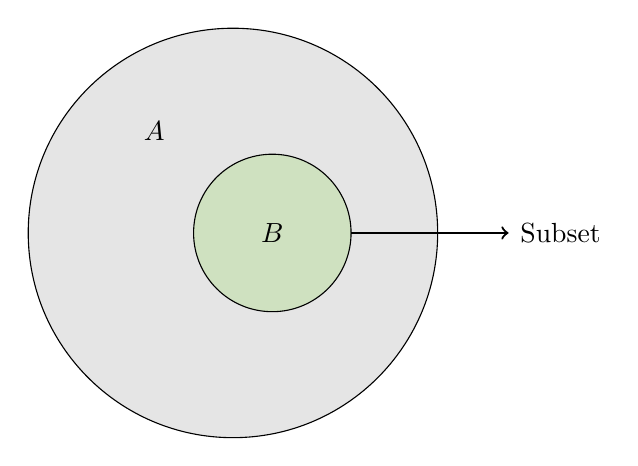
\begin{tikzpicture}
        % Set A
        \draw[fill=gray!20] (0,0) circle (2.6cm);
        \node at (-1,1.3) {$A$};

        % Set B
        \draw[fill=OliveGreen!20] (0.5,0) circle (1cm);
        \node at (0.5,0) {$B$};

        % Subset arrow
        \draw[->, thick] (1.5,0) -- (3.5,0);

        % Subset label
        \node at (4.16,0) {Subset};
    \end{tikzpicture}
    \caption{}
    \label{fig:subset}
\end{figure}


\noindent
Written $B \subseteq A$ or $A \supseteq B$, similar to the less than or
equal to signs `$\leq$' and `$\geq$'.

\begin{theo}[Subset]{thm:subset}
    If every element in set $B$ is also in set $A$, then $B$ is a subset of $A$.\\
    Denoted: $B \subseteq A$ or $A \supseteq B$.
\end{theo}

\noindent
\textbf{For Example:}
\begin{itemize}
    \item $\{-1, 0\} \subseteq \{-1, 0, 1, 2, 3\}$
    \item $\{-1, 1, 3\} \subseteq \{-1, 0, 1, 2, 3\}$
    \item $\{-1, 0, 1, 2, 3\} \subseteq \{-1, 0, 1, 2, 3\}$
    \item $\{-1, 7\} \not\subseteq \{-1, 0, 1, 2, 3\}$
\end{itemize}

\underline{$\not\subseteq$ denotes `not a subset of.'}

\vspace{1em}
\noindent
A set with no elements is called the empty set.
\begin{theo}[Empty Set]{thm:empty_set}
    Commonly denoted by $\emptyset$ or $\{\}$, refer to a collection with no objects.
\end{theo}

\noindent
\textbf{Questions:}
\begin{enumerate}
    \item How many elements are in the set  $\{\emptyset\}$?
    \item True or False: $\emptyset \subseteq \{\emptyset\}$.
    \item True or False: $\emptyset \in \{\emptyset\}$.
    \item True or False: $\emptyset \subseteq \emptyset$.
    \item True or False: $\emptyset \subseteq \mathbb{Z}$.
    \item True or False: $\emptyset \in \mathbb{Z}$.
\end{enumerate}

\noindent
\textbf{Answers:}
\begin{enumerate}
    \item 1 element, the empty set.
    \item True, the empty set is a subset of $\{\emptyset\}$.
    \item True, the empty set is an element of $\{\emptyset\}$.
    \item True, the empty set is a subset of itself.
    \item True, the empty set is a subset of all sets.
    \item False, the empty set is not an element of the integers.
\end{enumerate}

\noindent
\textbf{Why?} $\emptyset=\{\}$, A collection is an object, but this one just contains no objects.\\

\newpage
\noindent
Say we have an empty box. How many objects do we have? \textbf{Zero}.\\
Put an empty box inside our original box. How many objects now? \textbf{One}!


\begin{figure}[ht]
    $\hspace{.2cm}$
    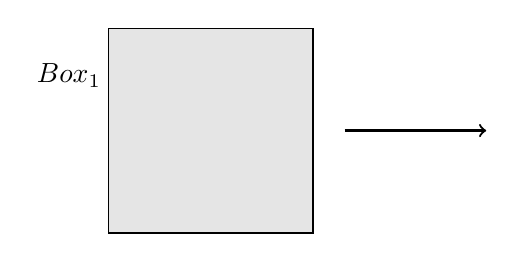
\begin{tikzpicture}
        % Set A
        \draw[fill=gray!20] (0,0) rectangle (2.6cm,2.6cm);
        \node at (-.5,2) {$Box_1$};

        % arrow
        \draw[->, thick] (3,1.3) -- (4.8,1.3);

    \end{tikzpicture}
    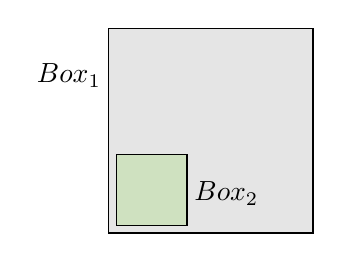
\begin{tikzpicture}
        % Set A
        \draw[fill=gray!20] (0,0) rectangle (2.6cm,2.6cm);
        \node at (-.5,2) {$Box_1$};

        % Set B
        \draw[fill=OliveGreen!20] (1,1) rectangle (.1cm,.1cm);
        \node at (1.5,0.5) {$Box_2$};

        \hfill
    \end{tikzpicture}
    \caption{\centering \underline{$Box_1$ contains \textbf{1} object,} which is $Box_2$ (an empty box). Hence $\quad$
        $Box_1$ represents $\{\{\}\}$ or $\{\emptyset\}$.}
    \label{fig:empty_box}
\end{figure}

\noindent
Counting the number of elements in a set is called the \textbf{cardinality} of the set.
\begin{theo}[Cardinality]{thm:cardinality}
    The number of elements in a set.\\
    Denoted over a set $A$ as $|A|$.
\end{theo}

\noindent
\textbf{For Example:}
\begin{itemize}
    \item $A = \{1, 2, 3\}$, $|A| = 3$.
    \item $B = \{a, e, i, o, u\}$, $|B| = 5$.
    \item $\mathbb{Z}$ the set of all integers, $|\mathbb{Z}| = \infty$.
\end{itemize}

\noindent
\textbf{Questions:}\\
What are the cardinalities of the following sets?
\begin{enumerate}
    \item $|\{1,2,3\}|$
    \item $|\emptyset|$
    \item $|\{\}|$
    \item $|\{\emptyset\}|$
    \item $|\{1,{2,3}\}|$
\end{enumerate}

\textbf{Answers:}
\begin{enumerate}
    \item 3
    \item 0
    \item 0
    \item 1
    \item 2
\end{enumerate}

\newpage

\noindent
Explicitly defining a set, say $\{1, 2, 3, ...\}$, is called \textbf{set-roster notation}.\\
\textbf{Set-builder notation} enables more complex definitions of a set.

\begin{theo}[Set-Builder Notation]{thm:set_builder}
    General form: $\{x \mid P(x)\}$,
    \begin{itemize}
        \item $x$ = defines some variable.
        \item $``\mid"$ = is short hand for ``such that.''
        \item $P(x)$ = describes the properties $x$ must satisfy.
    \end{itemize}
\end{theo}

\noindent
\textbf{For Example:} Lets define the set of even integers\\
\vspace{-1em}
\begin{itemize}
    \item $\{x \mid x \textnormal{ is an even integer}\}$: ``$x$, such that, $x$ is an even integer.''
    \item $\{x \in \mathbb{Z} \mid x \textnormal{ is even}\}$: ``$x$ in Integers, such that, $x$ is an even.''
    \item $\{x \in \mathbb{Z} \mid x \textnormal{ is not odd}\}$: ``$x$ in Integers, such that, $x$ is not odd.''
\end{itemize}

\noindent
\underline{\textbf{It's important to define exactly what variables are.}}
In the above, $x$ was stated directly as an integer. If not, x could be \underline{\textbf{water-balloons} or \textbf{puppies}.}
